\documentclass[conference]{IEEEtran}
\usepackage{cite}
\usepackage{graphicx}
\usepackage{placeins}
\usepackage{caption}
\usepackage{tabto}
\usepackage{subfigure}
\usepackage{enumerate}
\usepackage{afterpage}
\usepackage[font={small}]{caption}
\AtBeginDocument{\renewcommand{\abstractname}{Resumo}}
\begin{document}
\title{Projeto 3 de Princ\'ipios de Vis\~ao Computacional}
\author{\IEEEauthorblockN{Gabriel Martins de Miranda}
\IEEEauthorblockA{130111350\\
Universidade de Bras\'ilia\\
Email:gabrielmirandat@hotmail.com}
}
\maketitle
\begin{abstract}
A presente demonstra\c{c}\~ao se baseia no algoritmo de oito pontos de Hartley. Foram realizadas duas abordagens. A primeira implementou
o algoritmo n\~ao normalizado, enquanto que a segunda usou a fun\c{c}\~ao pronta do opencv que implementa o algoritmo de Hartley
normalizado. O objetivo do projeto \'e visualizar as retas epipolares encontradas a partir da matriz fundamental que relaciona 
as imagens $mantle1$ e $mantle2$ dados oito pontos de correspond\^encia entre elas.
\end{abstract}

\section{ Introdu\c{c}\~ao} 
\label{sec:meth} 
	Seguem alguns conceitos importantes para o entendimento do leitor:
	
	$cameraMatrix$: conhecida como $K$, \'e uma matriz $3$x$3$ que cont\'em informa\c{c}\~oes dos par\^ametros intr\'insecos
	da c\^amera. Quando multiplicada pela $poseMatrix$, matriz $3$x$4$ formada da concatena\c{c}\~ao das matrizes de rota\c{c}\~ao
	 e transla\c{c}\~ao da cena, forma a $projectionMatrix$, matriz $3$x$4$ que relaciona pontos numa imagem 2D com seus correspondentes
	 pontos 3D em coordenadas do mundo.
	 
	$fundamentalMatrix$: conhecida por $F$, \'e uma matriz $3$x$3$ que relaciona pontos correspondentes entre imagens
	est\'ereo. Pode ser estimada com no m\'inimo sete pontos de correspond\^encia. Ela \'e obtida quando n\~ao s\~ao 
	conhecidos os par\^ametros intr\'insecos da c\^amera, ou seja, a matriz $K$.
	
	$essentialMatrix$: conhecida por $E$, assim como a matriz $F$, \'e uma $3$x$3$ que relaciona pontos correspondentes
	em imagens est\'ereo assumindo c\^amera pinhole. Ao contr\'ario da $fundamentalMatriz$, $E$ \'e obtida quando os 
	par\^ametros intr\'insecos da c\^amera s\~ao conhecidos e s\~ao necess\'arios somente 5 par\^ametros, sendo 3
	de rota\c{c}\~ao e 2 de transla\c{c}\~ao.
	
	A equa\c{c}\~ao que relaciona as matrizes fundamental e essencial \'e dada por:
	$F$ = $K^{-T}EK'^{-1}$, onde $K$ \'e a $cameraMatrix$ relacionada \`a primeira c\^amera e $K'$ \'e a $cameraMatrix$ 
	relacionada \`a segunda c\^amera.
	
	$rank\> de\> uma\> matriz$: para definir o conceito de $rank$ de uma matriz, primeiro definiremos os conceitos de $row$ $rank$
	e $column$ $rank$. Seja $A$ uma matriz $m$x$n$ qualquer. Assim, temos que o $row$ $rank$ de $A$ \'e o n\'umero m\'aximo
	de linhas linearmente independentes de A, ou seja, linhas que n\~ao podem ser obtidas por combina\c{c}\~ao linear de 
	umas com as outras. Intuitivamente, o $column$ $rank$ de $A$ \'e o n\'umero m\'aximo de colunas linearmente independentes
	 de A. Como $A$ possui $m$ linhas e $n$ colunas, $row$ $rank$ de $A$ $<=$ $m$ e $column$ $rank$ de $A$ $<=$ $n$.Por\'em, 
	 temos que $row$ $rank$ de $A$ $=$ $colums$ $rank$ de $A$ sempre!! Logo, falamos de rank da matriz. Ent\~ao tiramos que
	 rank($A_{mxn}$) $<=$ min($m,n$).Atra\'ves de opera\c{c}\~oes entre as linhas, achamos a matriz minimizada. O n\'umero
	 de linhas diferente de zero \'e o $rank \> da \> matriz$.
	 
	$Singular\> Value\> Decomposition\>(SVD)$: \'e a fatoriza\c{c}\~ao de uma matriz real ou complexa. Tomando por exemplo
	a mesma matriz $A$ $m$x$n$ usada anteriormente, o SVD de A \'e $A=\> U\Sigma V^{T}$, em que $U$ \'e $m$x$m$ e ortogonal 
	(ou seja, sua transposta coincide com sua inversa), $V$ \'e $n$x$n$ e tamb\'em ortogonal e $\Sigma$ \'e uma matriz
	diagonal $m$x$n$ com entradas diagonais n\~ao negativas dadas por $\sigma{1}>=\sigma_{2}>=...>=\sigma_{p}$, em que $p$
	 = min($m,n$). Estes valores s\~ao conhecidos como valores singulares de $A$. O SVM \'e uma decomposi\c{c}\~ao extremamente 
	 \'util que produz muitas informa\c{c}\~oes sobre $A$, incluindo seu range, rank e espa\c{c}o nulo. Al\'em disto, 
	 podemos obter caracter\'isticas \'uteis da \'algebra linear no SVD. A saber, as $m$ colunas de $U$ e $n$ colunas de $V$ s\~ao os
	 chamados vetores singulares esquerda e vetores singulares direta de A, respectivamente. Os vetores singulares esquerda de $A$ s\~ao
	 autovetores de $AA$*. Os vetores singulares direita de $A$ s\~ao autovetores de $A$*$A$, e por fim, os valores singulares 
	 diferentes de zero de $A$ s\~ao as ra\'izes dos autovalores diferentes de zero de ambas $A$*$A$ e $AA$*.
	 \\
	 \\
	 \\
	 Diante do que foi explicitado, podemos finalmente entender como funciona o algoritmo de 8-pontos para c\'alculo da 
	 $matriz\> fundamental$.
	
\section{Metodologia} 
\label{sec:meth} 
     De maneira geral, os passos para a realiza\c{c}\~ao do algoritmo de 8-pontos s\~ao:
\begin{itemize}
  \item solu\c{c}\~ao de m\'inimos quadrados usando $SVD$ nas equa\c{c}\~oes dos oito pares de correspond\^encias. Daqui temos 
  uma primeira estimativa para $F$, que chamaremos de $F\sim$.
  \item Otimizar $F\sim$ for\c{c}ando a restri\c{c}\~ao de que a matriz fundamental $F$ \'e rank 2, o que implica 
  que det($F$) = 0. Para isto, usamos o $SVD$ na pr\'opria $F\sim$. O resultado \'e a matriz fundamental $F$ que procuramos.\\
\end{itemize}

 Nos aprofundando mais neste algoritmo, temos o seguinte:
 \\
 \\
 1) Resolver um sistema de equa\c{c}\~oes lineares.
	  \begin{itemize}
	   \item Escrever o sistema de equa\c{c}\~oes 
		  \\
		  \centering $x^{T}Fx'=0$ 
		  \\
		  Abrindo esta equa\c{c}\~ao, ficamos com
		  \\
		  \centering
		  $x'xf_{11}+x'yf_{12}+x'f_{13}+y'xf_{21}+y'yf_{22}+y'f_{23}+xf_{31}+yf_{32}+f_{33}$
		  \\
		  de onde tiramos a seguinte multiplica\c{c}\~ao matricial $(lembrando\> que\> devemos\> fazer\> para\> 
		  todos\> os\> 8\> pontos)$
		  
	  \end{itemize}
\footnotesize 
\[ \left( \begin{array}{ccccccccc}
x'_{1}x_{1} & x'_{1}y_{1} & x'_{1} & y'_{1}x_{1} & y'_{1}y_{1} & y'_{1} & x_{1} & y_{1} & 1 \\
x'_{2}x_{2} & x'_{2}y_{2} & x'_{2} & y'_{2}x_{2} & y'_{2}y_{2} & y'_{2} & x_{2} & y_{2} & 1 \\
x'_{3}x_{3} & x'_{3}y_{3} & x'_{3} & y'_{3}x_{3} & y'_{3}y_{3} & y'_{3} & x_{3} & y_{3} & 1 \\
x'_{4}x_{4} & x'_{4}y_{4} & x'_{4} & y'_{4}x_{4} & y'_{4}y_{4} & y'_{4} & x_{4} & y_{4} & 1 \\
x'_{5}x_{5} & x'_{5}y_{5} & x'_{5} & y'_{5}x_{5} & y'_{5}y_{5} & y'_{5} & x_{5} & y_{5} & 1 \\
x'_{6}x_{6} & x'_{6}y_{6} & x'_{6} & y'_{6}x_{6} & y'_{6}y_{6} & y'_{6} & x_{6} & y_{6} & 1 \\
x'_{7}x_{7} & x'_{7}y_{7} & x'_{7} & y'_{7}x_{7} & y'_{7}y_{7} & y'_{7} & x_{7} & y_{7} & 1 \\
x'_{8}x_{8} & x'_{8}y_{8} & x'_{8} & y'_{8}x_{8} & y'_{8}y_{8} & y'_{8} & x_{8} & y_{8} & 1 
\end{array} \right)
\left( \begin{array}{c}
f_{11} \\
f_{12} \\
f_{13} \\
f_{21} \\
f_{22} \\
f_{23} \\
f_{31} \\
f_{32} \\
f_{33}
\end{array} \right)
= 0
\]
\normalsize
\tab $ou$
\tab $Af = 0$


\begin{itemize}
	   \item Resolver $f$ de $Af$=0 usando $SVD$. A primeira estimativa de $F$, a $F\sim$, \'e obtida da matriz $V^{T}$
	   da decomposi\c{c}\~ao $SVD$ de $A$. A \'ultima linha de nove elementos de $V^{T}$ corresponde aos nove elementos 
	   de $F\sim$ distrib\'idos em $3$x$3$.
\end{itemize}		  
		
		\vspace{2\baselineskip}\vspace{-\parskip}
		\begin{minipage}{\linewidth}
  		\centering
  		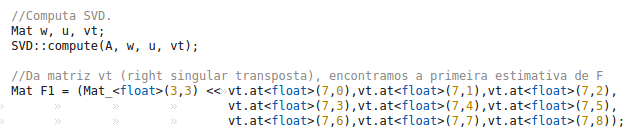
\includegraphics[width=3.5in]{svd1_ok}
  		\captionof{figure}{Estimativa de $F\sim$.}
		\end{minipage}
	  
\vspace{2\baselineskip}\vspace{-\parskip}
2) Resolver a restri\c{c}\~ao que det($F$)=0, usando o $SVD$.
\begin{itemize}
 \item Precisamos for\c{c}ar a restri\c{c}\~ao de singularidade.
 \\
 A matriz fundamental tem rank 2: det($F$)=0
 \\
 Fazer com que as linhas epipolares coincidem num mesmo ponto.
\end{itemize}

		
		\vspace{2\baselineskip}\vspace{-\parskip}
		\begin{minipage}{\linewidth}
  		\centering
  		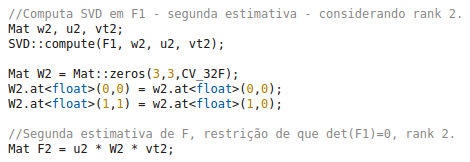
\includegraphics[width=3.5in]{svd2}
  		\captionof{figure}{Estimativa de $F$.}
		\end{minipage}

\vspace{2\baselineskip}\vspace{-\parskip}
3) Um adicional importante que se pode fazer \'e resolver o algoritmo em sua forma $normalizada$, j\'a que n\~ao foram 
considerados fatores de escala. Para isto podemos apenas chamar a fun\c{c}\~ao pronta do opencv especificando a flag 
$CV\_FM\_8POINT$, que calcula o algoritmo de 8-pontos normalizado de Hartley.
\\
\begin{itemize}
 \item Normalizamos as coordenadas da imagem com $\tilde{x}$ = $Tx$ e $\tilde{x'}$ = $T'x'$ 
 \item Desnormalizamos as coordenadas da imagem com $F$ = $T'^{-1}\tilde{F}T$
\end{itemize}

		\vspace{2\baselineskip}\vspace{-\parskip}
		\begin{minipage}{\linewidth}
  		\centering
  		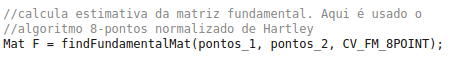
\includegraphics[width=3.5in]{pronta}
  		\captionof{figure}{Estimativa de $F$ com algoritmo de 8-pontos normalizado.}
		\end{minipage}


\section{Resultados} 
\label{sec:meth} 
1) Aqui s\~ao mostrados os resultado obtidos e a estimativa das retas epipolares:

		\vspace{2\baselineskip}\vspace{-\parskip}
		\begin{minipage}{\linewidth}
  		\centering
  		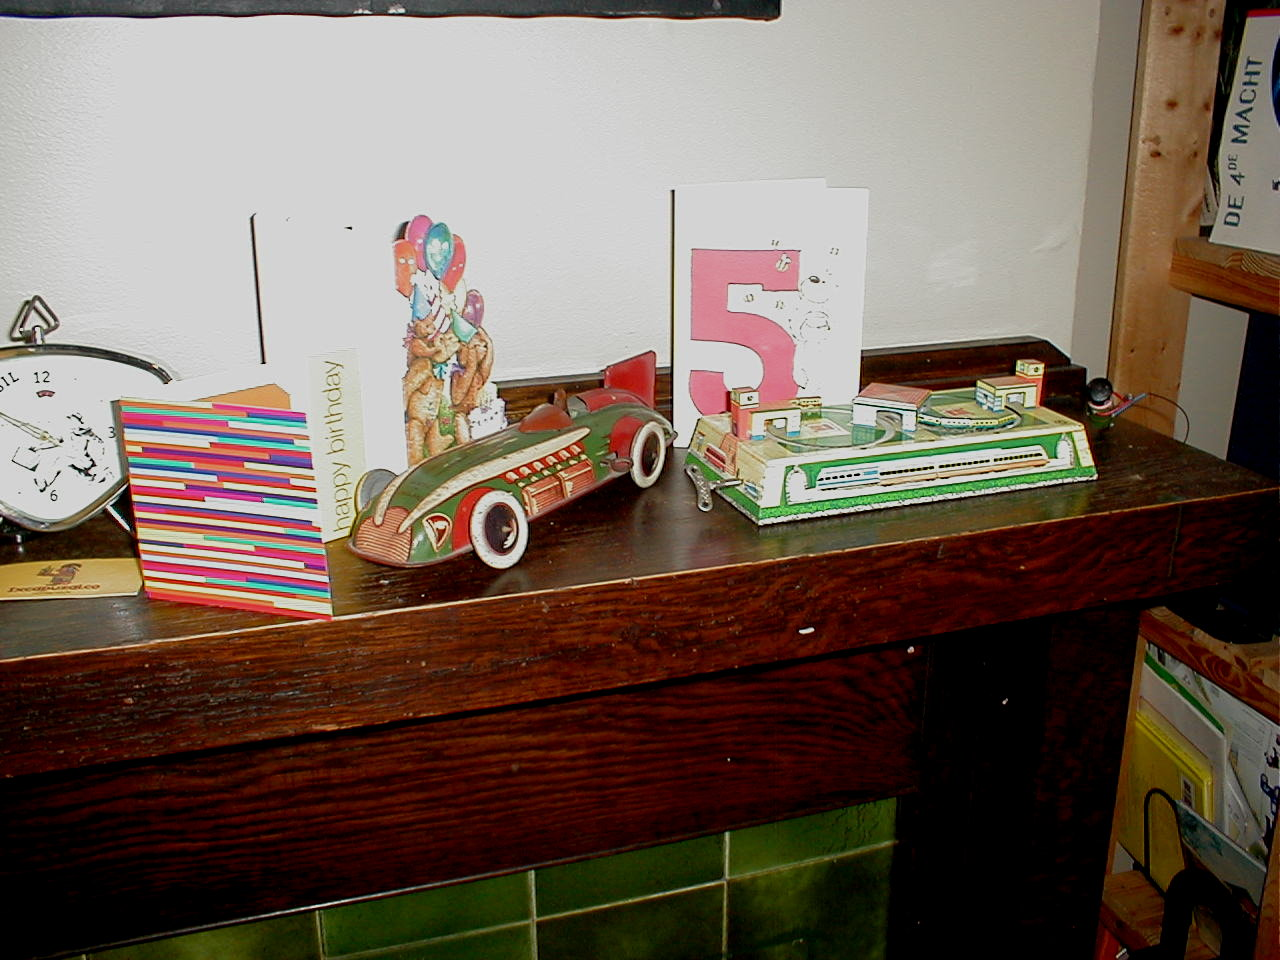
\includegraphics[width=3.3in]{mantle1}
  		\captionof{figure}{imagem mantle1.}
		\end{minipage}
		
		\vspace{2\baselineskip}\vspace{-\parskip}
		\begin{minipage}{\linewidth}
  		\centering
  		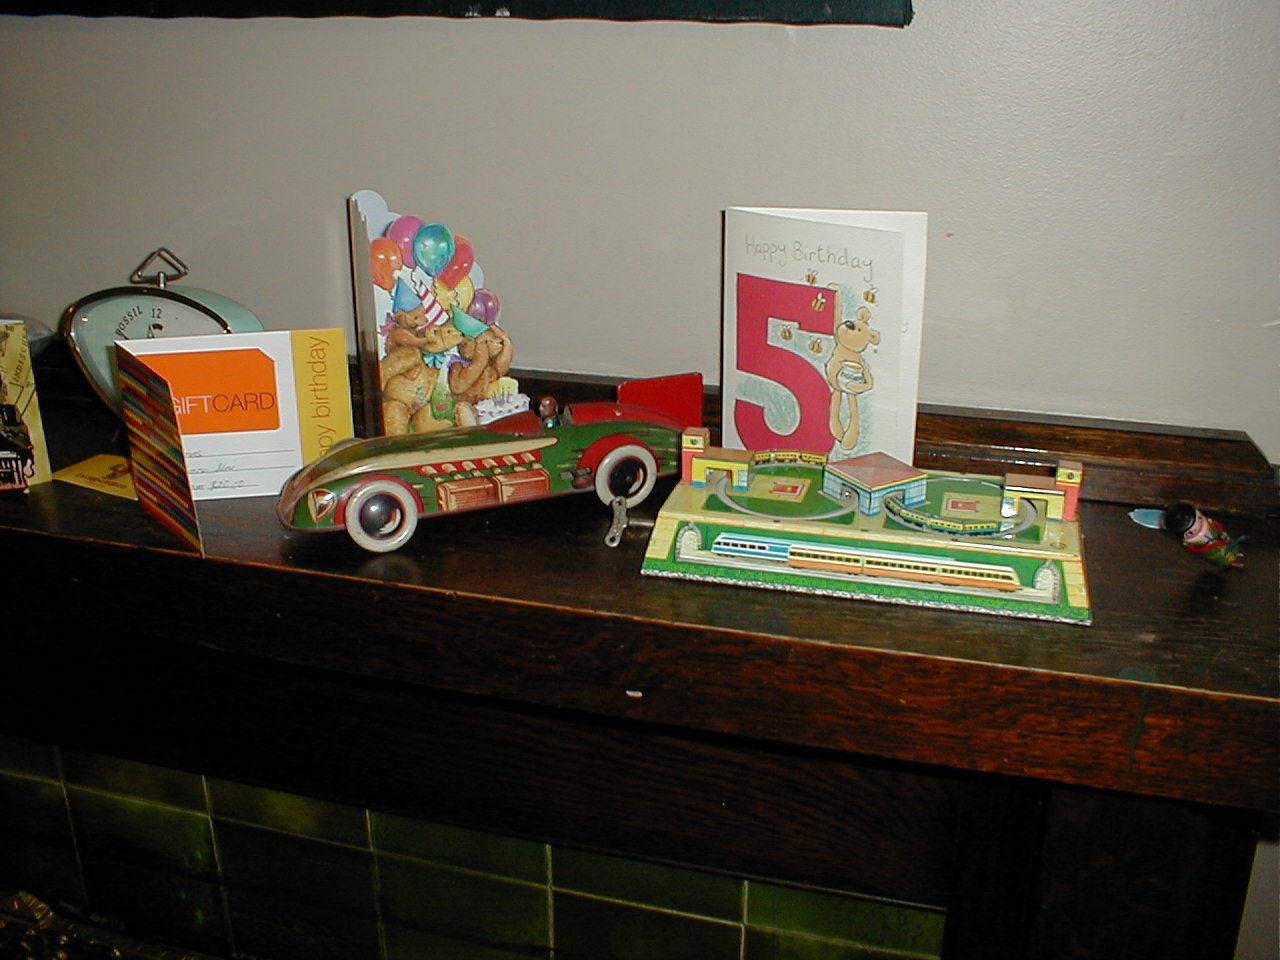
\includegraphics[width=3.3in]{mantle2}
  		\captionof{figure}{imagem mantle2.}
		\end{minipage}
		
		\vspace{2\baselineskip}\vspace{-\parskip}
		\begin{minipage}{\linewidth}
  		\centering
  		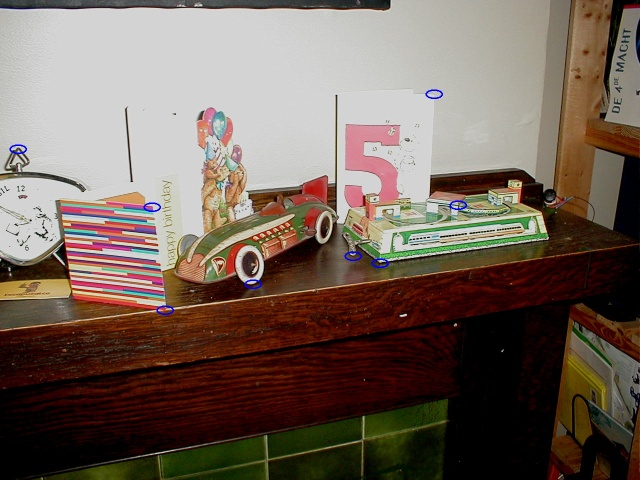
\includegraphics[width=3.3in]{pontos_im1}
  		\captionof{figure}{8 pontos de correspond\^encia de mantle1.}
		\end{minipage}
		
		\vspace{2\baselineskip}\vspace{-\parskip}
		\begin{minipage}{\linewidth}
  		\centering
  		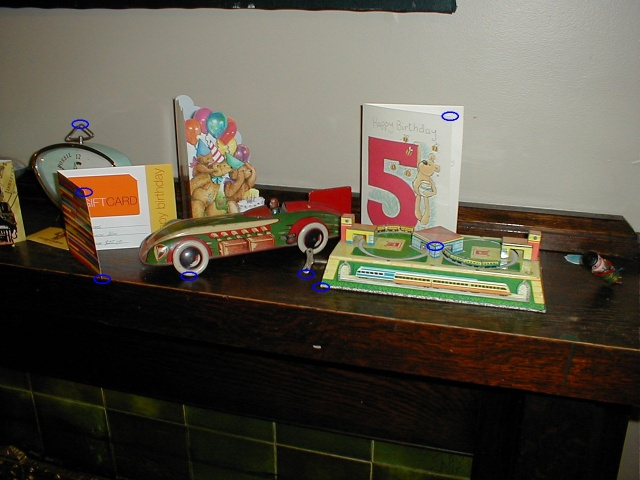
\includegraphics[width=3.3in]{pontos_im2}
  		\captionof{figure}{8 pontos de correspond\^encia de mantle2.}
		\end{minipage}

		
		\vspace{2\baselineskip}\vspace{-\parskip}
		\begin{minipage}{\linewidth}
  		\centering
  		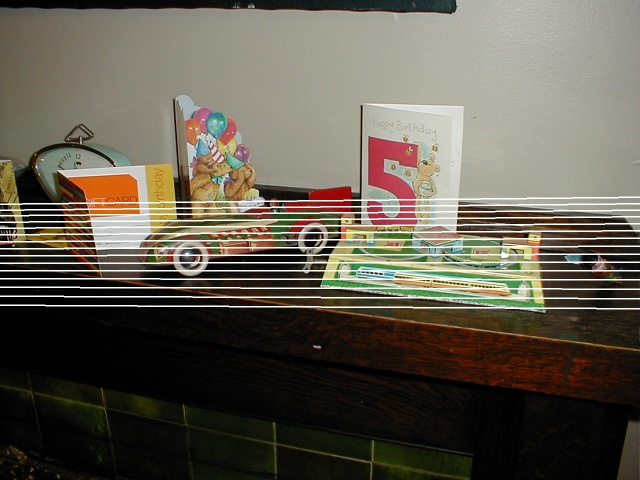
\includegraphics[width=3.3in]{img2epiF1}
  		\captionof{figure}{epipolares sem restri\c{c}\~ao rank2 n\~ao normalizado.}
		\end{minipage}
		
		\vspace{2\baselineskip}\vspace{-\parskip}
		\begin{minipage}{\linewidth}
  		\centering
  		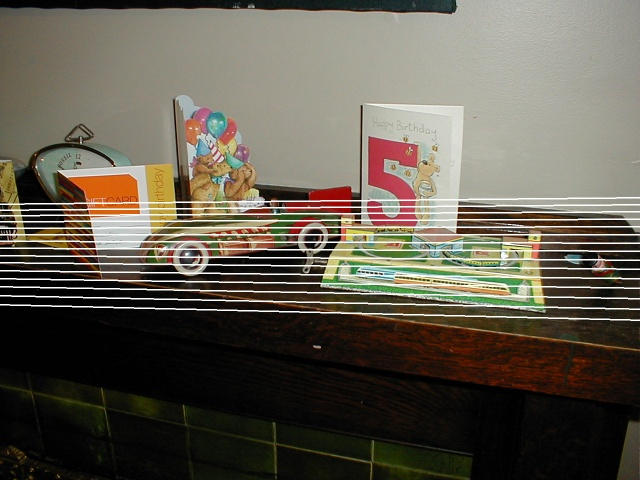
\includegraphics[width=3.3in]{img2epiF2}
  		\captionof{figure}{epipolares com restri\c{c}\~ao rank2 n\~ao normalizado.}
		\end{minipage}

		
		\vspace{2\baselineskip}\vspace{-\parskip}
		\begin{minipage}{\linewidth}
  		\centering
  		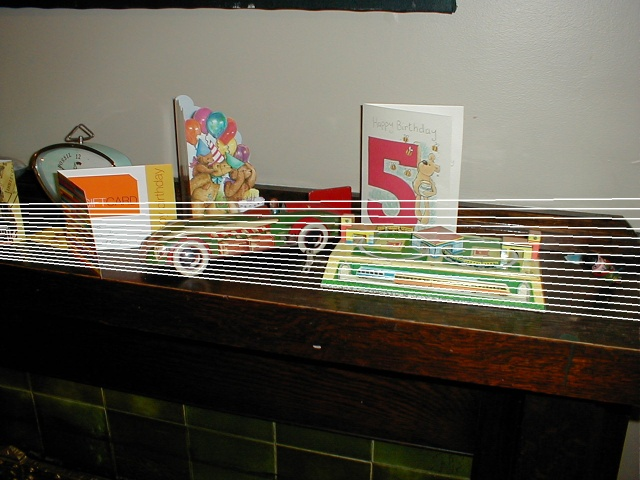
\includegraphics[width=3.3in]{img2epi}
  		\captionof{figure}{epipolares com restri\c{c}\~ao e normalizado.}
		\end{minipage}	

	
\section{Conclus\~ao} 
\label{sec:meth} 

Atrav\'es do algoritmo aqui proposto, \'e poss\'ivel obter uma boa estimativa para as retas epipolares atrav\'es da 
matriz fundamental encontrada pelo m\'etodo de Hartley. Foi poss\'ivel perceber que h\'a uma grande diferen\c{c}a 
em se tratando do algoritmo n\~ao-normalizado com o normalizado, que foi bem mais preciso. 

\section{Refer\^encias} 
\label{sec:meth} 

[1] http://robotics.stanford.edu/~birch/projective/node20.html

[2] http://answers.opencv.org/question/27155/from-fundamental-matrix-to-rectified-images/

[3] http://answers.opencv.org/question/38340/estimate-camera-pose-
extrinsic-parameters-from-homography-essential-matrix/

[4] https://www8.cs.umu.se/kurser/TDBD19/VT05/reconstruct-4.pdf

[5] http://web.mit.edu/be.400/www/SVD/Singular\_Value\_
Decomposition.htm

[6] http://www.hasper.info/opencv-draw-epipolar-lines/

[7] http://www.cs.utexas.edu/users/inderjit/public\_papers/
HLA\_SVD.pdf

[8] http://docs.opencv.org/master/da/de9/tutorial\_py\_
epipolar\_geometry.html

[9] http://www.cliffsnotes.com/math/algebra/linear-algebra/real-euclid
ean-vector-spaces/the-rank-of-a-matrix

[10] http://answers.opencv.org/question/36751/kmeans-clustering-for-vec
torpoint2f-data-structure/

[11] http://arxiv.org/pdf/1403.4806.pdf

[12] http://www.quora.com/Why-is-the-fundamental-matrix-in-computer-visi
on-rank-2

[13] http://en.wikipedia.org/wiki/Fundamental\_matrix\_
%28computer\_vision%29

[14] http://www.emgu.com/wiki/files/1.3.0.0/html/55d6f4d2-223d-8c55-
2770-2b6a9c6eefa2.htm

[15] http://stackoverflow.com/questions/12029486/matlab-svd-output-
in-opencv

[16] http://en.wikipedia.org/wiki/Singular\_value\_
decomposition\#Applications\_of\_the\_SVD

[17] https://www.youtube.com/watch?v=JEYLfIVvR9I

[18] http://docs.opencv.org/master/df/df7/classcv\_1\_
1SVD.html\#details

[19] http://websites.uwlax.edu/twill/svd/svd/index.html

[20] http://web.stanford.edu/class/cme335/lecture6.pdf

[21] http://www.cs.carleton.edu/cs\_comps/0607/recommend
/recommender
/svd.html

[22] http://en.wikipedia.org/wiki/Singular\_value
\_decomposition

[23] http://citeseerx.ist.psu.edu/viewdoc/summary
?doi=10.1.1.114.2762


\end{document}